\chapter{Arhitectura aplicației}

În mare parte aplicația este construită în jurul unei singure scene folosind $Unity$, arhitectura aplicației depinzând în mare parte de uneltele disponibile în motorul grafic și modul în care acesta funcționează Am încercat să împart căt de mult se poate să împart aplicația în module cu o coeziune căt mai ridicată. De acceea sistemul de instanțiere, generare și amplasare a obiectelor este construit cu principalul scop de a fi modular. Chiar și librăria ce modelează prototipul Markov cu stări invizibile este decuplat de algoritmul de antrenare în sine, putând fi schimbat oricând fără repercursiuni.\par

Aplicația folosește și multe funcții de $callback$ pentru a determina cănd anumite elemente din cadrul jocului ar trebui activate. Spre exemplu cea mai folosită funcție este cea de $OnTriggerEnter$, ce determină cănd un $RigidBody$\footnote{Componenta ce determina daca obiectul este supus motorului de fizica} se intersectează cu un \textit{Box}\textit{Collider}\footnote{Componenta ce determina zona de coliziune a unui obiect}.\par

\begin{lstlisting}[caption=Exemplu de utilizare a functiei OnTriggerEnter]
void OnTriggerEnter(Collider collidingObject){
        if (!this.triggered){
            this.callbackObject.GetComponent<PlatformBuilder>().InstantiatePlatform();
            this.triggered = true;
        }
}
\end{lstlisting}
\par

De asemena $Unity$ dispune de o unealtă foarte utilă numită $Inspector$ ce permite asignarea de referințe a obiectelor din scenă în scripturi, lucru foarte util și eficient atunci cănd este necesară legarea anumitor module. De exemplu $callbackObject$ reprezintă obiectul din scenă de care este atașat codul sursă ce se ocupă de construirea platformelor, numit sugestiv $PlatformBuilder$, din care se apelează funcția $IntantiatePlatform$ destinată acestui scop.\par

\section{Detalii legate de implementarea librăriei}

\vspace{10mm}
\begin{figure}[H]
\centering
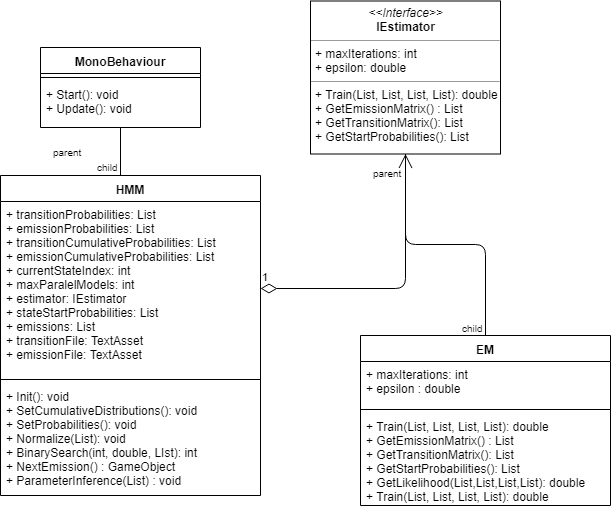
\includegraphics[width=0.65\linewidth]{HMM.png} \par
\caption{Diagrama UML ce modeleaza libraria de HMM}
\end{figure}

\section{Detalii legate de implementarea sistemului de instanțiere}

\section{Utilizarea librăriei în joc}

\section{Detalii legate de aspectul aplicatiei}

\section{Structura întregii aplicații}